\section{Introducción}

La obtención de una métrica que permita determinar la calidad de un proyecto considerando
los nombres de los indicadores que forman parte del mismo, es un proceso complejo y compuesto
por diferentes etapas, tal como se muestra en la figura X.
En primera instancia, podemos establecer que el proceso como un todo se divide en dos fases:
fase de cálculo y fase de visualización.

\begin{figure}[H]
    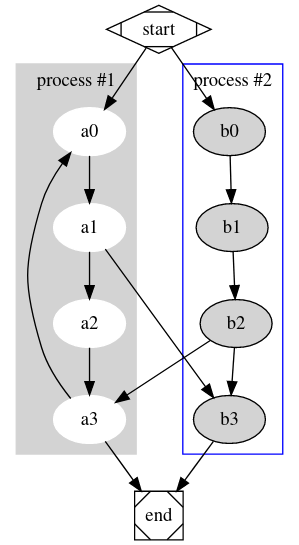
\includegraphics[height=8cm]{implementation/phases.png}
    \centering
    \caption{Fases y etapas}
  \end{figure}

La primera fase tiene el objetivo de calcular, por cada indicador considerado, cuál es el
valor de la métrica.
Para ello, esta fase se divide a su vez en diferentes etapas: extracción, procesamiento y
cálculo.

Dentro de la fase de cálculo, la etapa de extracción tiene por objetivo acceder al repositorio
de código fuente, y luego iterar sobre cada uno de los archivos para armar los árboles de sintáxis
abstracta.
Estos ASTs (por su sigla en inglés), constituyen la entrada para la etapa de procesamiento.

En la etapa de procesamiento, se realizan diferentes acciones sobre los ASTs.
Algunos algoritmos requieren de información contextual o derivada del código fuente (tanto en
fragmentos como en su totalidad), por lo que existe un pre-procesamiento.
Luego, el resultado es empleado para la aplicación de los algormitmos encargados de la división
y expansión de los indicadores extraídos.

Por último, en la fase de cálculo, se lleva a cabo la etapa donde se realiza efectivamente
el cálculo de la métrica, para determinar qué tan distanciado está el nombre del indicador,
de su supuesta y más significativa expansión.

La segunda fase, correspondiente a la visualización, permite al usuario final acceder
a las métricas por indicador previamente obtenidas, en el contexto del proyecto, tanto sea
por el análisis de la misma a nivel de paquetes/proyecto, como también de su impacto en
el caso de reemplazar el código original con las modificaciones propuestas.
